\documentclass[12pt]{article}
\usepackage{graphicx}
\graphicspath{{images/}}
\author{Andrea Malvezzi}
\title{\textbf{Architettura degli Elaboratori - Introduzione}}
\date{19 Settembre, 2024}
\begin{document}
\maketitle
\section*{A cosa serve questo corso?}
L'architettura degli elaboratori cerca di spiegare il funzionamento dei calcolatori dal punto di vista dell'hardware \textit{(HW)}.
\section {La composizione dei calcolatori}
\subsection{Le porte logiche}
Un calcolatore è composto da migliaia di componenti, tra cui le \textbf{PORTE LOGICHE}.\\
Esistono diversi tipi di porte logiche, ma due di queste - la NAND e la NOR - nutrono di una peculiarità: queste sono dette "\textbf{UNIVERSALI}" in quanto combinandole tra loro è possibile produrre tutte le altre funzioni logiche (o \textit{booleane}).
\subsection{Il principio di Astrazione/Implementazione}
Per realizzare sistemi complessi partendo da queste porte si usa il \textbf{principio di "Astrazione/Implementazione"}:
\begin{itemize}
    \item Astrazione: si frammenta il problema di partenza in problemi minori, più semplici da risolvere.
    \item Implementazione: si realizza la soluzione al problema di partenza combinando tra loro le soluzioni minori precedentemente escogitate.
\end{itemize}
\pagebreak
\section{Elaboratori multilivello}
Un elaboratore può essere composto da più livelli e generalmente è corretto dire che i livelli superiori sono destinati alla rsoluzione di problemi mediante linguaggi adatti, mentre quelli inferiori sono improntati alla gestione delle risorse e alla comunicazione tra HW e SW.\\
\begin{figure}[!htb]
    \centering
    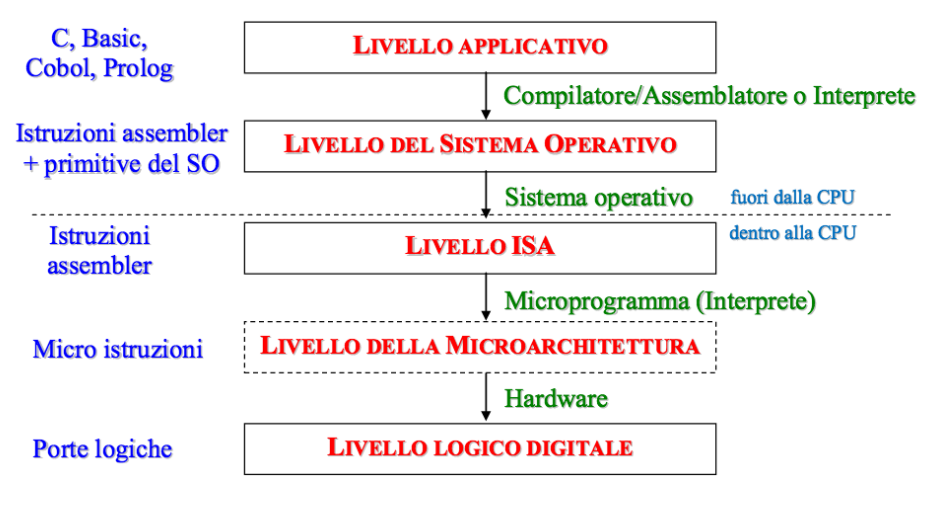
\includegraphics[width=.9\linewidth,height=.40\textheight,keepaspectratio]{introduzione/struttura_multilivello.PNG}
    \begin{center}
        \caption{Un esempio della struttura di un elaboratore a più livelli.}
    \end{center}
    \label{fig:es_1}
\end{figure}
\subsection{Livello 0: livello logico digitale}
Qui si hanno le porte logiche e conseguentemente è dove avvengono le relative operazioni.
\subsection{Livello 1: livello di microarchitettura}
La microarchitettura è ciò che in un elaboratore gestisce il flusso di dati tra i vari componenti.\\
Può trattarsi sia di HW che di SW.
\subsection{Livello 2: livello ISA(Instruction Set Architecture)}
Funge da interfaccia da HW e SW.\\
Contiene le istruzioni che vengono eseguite nella microarchitettura.
\subsection{Livello 3-4: O.S. e Assembly}
Qui si programmano i livelli sottostanti, si gestiscono le risorse del sistema e si eseguono i programmi.
\subsection{Livello 5: livello del linguaggio}
Qui è dove si usano linguaggi più vicini agli esseri umani per risolvere problemi e fornire servizi. Il codice di questi linguaggi dovrà essere tradotto in linguaggio macchina per essere eseguito. 
\end{document}